% Uds_xPass seminar report — build with: cd report && latexmk -pdf main.tex
\documentclass[11pt,a4paper]{article}
\usepackage[margin=25mm]{geometry}
\usepackage{graphicx}
\usepackage{booktabs}
\usepackage[T1]{fontenc}
\usepackage[hidelinks]{hyperref}
\usepackage{xurl}
\urlstyle{same}
\usepackage{amsmath}
\usepackage{caption}
\graphicspath{{../poster_outputs/}{../archive/single_season_2020_21/}}
\title{Can We Predict Every Pass?\\Weak-Foot Effects and Pass-Type Calibration in an xPass Model for La Liga}
\author{Aashish Nair (7086324) \and Ankit Khatiwada (7089529) \and Moaaz Sajjad Warraich (7089952)}
\date{Sports Analytics Seminar 2026}
\begin{document}
\maketitle

\begin{abstract}
Just as Expected Goals (xG) estimates the probability that a shot becomes a
goal, Expected Pass (xPass) estimates the probability that a pass is
completed given the state of play. We build an event-only XGBoost xPass
model on StatsBomb open data covering 18 La Liga seasons and more than
400\,000 passes, and investigate two questions that prior work largely
ignores: does a player's weak foot hurt pass completion, and is the model
equally well calibrated across different kinds of passes? Weak-foot passes
carry approximately 15--20\% lower completion odds after controlling for
pass difficulty, an effect that is significant in 13 of the 17 modern seasons (1973/74 excluded, n~=~555, wrong-signed). The
model discriminates well overall (per-season AUC 0.85--0.91) and is
near-perfectly calibrated on Ordinary passes (Expected Calibration Error,
ECE~=~0.003), but calibration degrades by up to a factor of 15 on rare
pass types (Through-ball ECE~=~0.043). A feature ablation shows small,
inconsistent footedness effects that move error between types rather than
removing it, and inverse-frequency reweighting of
rare types degrades calibration almost everywhere. Per-type isotonic recalibration fails on every rare type while leaving Ordinary untouched. An equal-n downsampling experiment shows Ordinary passes degrade roughly eightfold when starved to rare-type sample sizes, since most of the gap is scarcity and estimator noise, with a residual type-intrinsic penalty of up to $\sim$2$\times$ surviving matching. We conclude
that poor calibration on rare pass types is driven primarily by data
scarcity, with a smaller intrinsic component, rather than by missing footedness features, and that adding
player-specific technical attributes makes xPass more useful for player
evaluation, scouting, and tactical analysis.
\end{abstract}

\section{Introduction}
Passing is the most frequent on-ball action in football, yet raw completion
percentages are a poor measure of passing skill because they ignore
difficulty: a sideways five-metre pass under no pressure and a forty-metre
through ball between defenders are counted the same. Expected Pass (xPass)
addresses this by modelling the probability of completion conditional on
the characteristics of the pass and the surrounding game context. Like xG,
xPass separates decision quality from execution quality: a player
attempting difficult passes can be credited for ambition even when some
fail, while a player misplacing simple passes is penalised appropriately.
Applications include evaluating passing ability, scouting, and tactical
analysis.

This project began as a generalisation check: does an xPass model trained
in one competition transfer to another (the Women's Bundesliga pilot in
our proposal, Expected-Passs-in-Football.pptx)? The pilot
showed the model is strong globally but uneven locally, which motivated
the La Liga deep-dive that forms the core of this report. We add player
footedness, a potentially influential factor that has received little
attention in the xPass literature, scale the analysis across all La
Liga seasons available in StatsBomb's open data, and split evaluation by
pass type. The report follows that order: baseline model, footedness
hypothesis, pass-type calibration, ablation, and recalibration.

Our contributions are: (1) a controlled multi-season test of the
weak-foot effect; (2) pooled calibration analysis by pass type showing
that miscalibration scales with sample scarcity; (3) an ablation
demonstrating that footedness features help only marginally; and
(4) a recalibration experiment that uses the success pattern of isotonic
regression as a diagnostic for the scarcity hypothesis.

\section{Related work}
Szczepa\'nski and McHale (2016) showed that raw completion rates are
limited because they ignore pass difficulty, motivating difficulty-aware
evaluation. Anzer and Bauer (2022) formalised the Expected Pass framework,
modelling pass difficulty as completion probability from spatio-temporal
context; their feature set is the direct template for ours. Robberechts et
al.\ (2023) extended pass evaluation toward creativity (valuable and
atypical passes), relevant to risk--reward analysis. On the modelling
side, Arbu\'es-Sang\"uesa et al.\ (2020) demonstrated that player body
orientation and opponent positioning affect pass feasibility: features
we approximate with 360 freeze-frame data where available and otherwise
list as limitations. Rahimian et al.\ (2024) predicted receivers and
outcomes with temporal graph networks, pointing toward sequential
extensions, and Takamido et al.\ (2025) applied explainable machine
learning to multimodal match data for pass outcome classification,
relevant to interpretability. None of these foreground the weak-foot
effect or stratify calibration by pass type, which is the gap we address.

\section{Data}
We use StatsBomb open-data events for every men's La Liga season on
record: 1973/74 plus 2004/05 through 2020/21. Early seasons are mostly
Messi-era Barcelona matches (roughly 30--40 games per season); 2015/16 is
far larger (307\,973 usable passes) and 2020/21 is a full season. Raw
events are cached to \url{data/passes_<season_id>.parquet} (or .pkl where pyarrow is
unavailable) so re-runs avoid re-pulling. The 2020/21 season additionally
provides 360 freeze-frame data, used only for the event-only versus
360-enriched bonus comparison. Two caveats apply throughout. First,
pass-cut-back never populates in this pull (zero variance), so
cut-backs are excluded from type-level analyses and dropped from the
per-season logit controls. Second, 1973/74 contributes only 555 passes
with incomplete body-part tagging and a positive logit coefficient; it is
retained in tables for transparency but excluded from headline claims.

\section{Methods}

\subsection{Preferred-foot inference and validation}
StatsBomb provides the body part used for each pass but no ground-truth
preferred foot. We infer it per season from pass volume: a player's share
of Right-foot passes at or above 0.55 (at or below 0.45) labels them Right
(Left), otherwise Both, with players under 20 footed attempts left
unlabelled. Inference is per season because squads and minutes shift. A
pass is flagged weak-foot~=~1 when the foot used differs from
the inferred preferred foot. For 2020/21 we validate the inference
against FIFA 21 preferred-foot labels
(\url{preferred_foot_fifa.csv}, fuzzy name matching; raw dump
\url{players_21.csv}). The broader source search across FBref,
Transfermarkt, FIFA, and Wikidata is frozen in \url{archive/} for
provenance; the final pipeline uses usage-inferred foot at scale with the
FIFA check as validation.

\subsection{Feature engineering}
Table~\ref{tab:feats} lists the 24 event-only features (Anzer and Bauer 2022 template plus footedness). Geometry and goal-context features capture pass difficulty; length buckets and height capture trajectory; type flags and pressure capture context; footedness and its interactions capture execution. The ablation in \S\ref{sec:ablation} varies only the footedness group: no-footedness drops weak-foot and wf-cross; current keeps both; full-interactions adds wf-switch and wf-through-ball (26 features). pass-cut-back is zero-variance in this pull and retained only as a placeholder. The 360-enriched variant (2020/21 only) adds six freeze-frame features described in the bonus section.
\begin{table}[h]
\centering
\small
\begin{tabular}{lp{9cm}c}
\toprule
Group & Features & $n$ \\
\midrule
Geometry & pass length, pass angle, forward progress, lateral distance, pass direction, start x/y $\rightarrow$ zone x, zone y & 7 \\
Goal context & distance to goal, end distance to goal, distance to sideline, angle to goal & 4 \\
Length / height & length short, length medium, length long, height & 4 \\
Context / type & under pressure, cross, switch, through ball, cut back & 5 \\
Footedness & weak foot, weak foot $\times$ cross & 2 \\
Interactions & pressure $\times$ length, cross $\times$ pressure & 2 \\
\midrule
Total event-only & & 24 \\
Ablation extras & weak foot $\times$ switch, weak foot $\times$ through ball (full interactions only) & +2 \\
360-only bonus & closest-defender distances (passer/receiver), defenders in lane, visible opponents/teammates, defenders behind passer & +6 \\
\bottomrule
\end{tabular}
\caption{Event-only feature set by group. The ablation varies only the footedness group; all other groups are identical across variants.}
\label{tab:feats}
\end{table}

\subsection{Features and model}
The event-only feature set follows Anzer and Bauer (2022) as detailed in Table~\ref{tab:feats} (24 features total). We train one XGBoost
classifier per season (n-estimators=400, max-depth=5,
learning-rate=0.05, subsample=colsample-bytree=0.8,
min-child-weight=5, gamma=1.0, reg-alpha=1.0) on a match-level 80/20
split with seed 42, so no match appears in both train and test. The
360-enriched variant adds six freeze-frame features (closest-defender
distances to passer and receiver, defenders in the passing lane, visible
opponents/teammates, defenders behind the passer) for 2020/21 only.

\subsection{Evaluation}
Discrimination is measured by AUC; probability quality by Brier score and
Expected Calibration Error (ECE, 10 bins). The weak-foot hypothesis is
tested per season with (i) the raw strong-versus-weak completion gap,
(ii) a $\chi^2$ test of independence, and (iii) the coefficient on
weak-foot in a logistic regression controlling for length,
pressure, type flags, distance and angle to goal. Zero-variance controls
are dropped per season and a regularised-sklearn fallback with bootstrap
confidence intervals is used if the statsmodels fit fails, so no season
is silently dropped. For the ablation we train three variants that differ
only in footedness features (no-footedness drops weak-foot and wf-cross; current keeps both; full-interactions adds wf-switch and wf-through-ball) and compare Brier/ECE per
pass type on pooled held-out predictions. A follow-up weighting experiment
(\url{weighted_study.py}) trains the same model with sample weights
emphasising rare types (unweighted ($w=1$),
inv-type ($w \propto 1/\mathrm{frequency}$), and a milder
sqrt-inv-type) on the five largest cached seasons. An equal-n downsampling experiment
(\url{downsample_study.py}) isolates the scarcity component: it repeatedly subsamples the pooled Ordinary predictions to each rare type's exact n (200 resamples) and recomputes ECE/Brier, separating sample size and estimator noise from type-intrinsic effects. For recalibration we fit
per-type isotonic regression on one half of the pooled held-out
predictions and evaluate before/after calibration on the other half, so
the ``after'' numbers cannot reflect fit-set overfitting.

\section{Results}

\subsection{Finding 1: weak-foot passes complete less often}
Figure~\ref{fig:forest} shows the controlled weak-foot logistic
coefficient per season with 95\% confidence intervals. The coefficient is
negative in all 17 modern seasons, ranging from about $-0.06$ to $-0.40$ (median $-0.17$),
corresponding to typically 15--20\% lower completion odds at fixed
difficulty, and is statistically significant in 13 of the 17 modern seasons (1973/74 excluded). The
2015/16 estimate is the most precise ($-0.184$, $p < 10^{-41}$,
n~=~307\,973). Raw gaps are smaller (typically 0--4 percentage points)
because weak-foot passes tend to be attempted in easier situations, which
is precisely why the controlled coefficient, not the raw gap, is
the quantity of interest. Full per-season statistics are in
\url{weak_foot_hypothesis_by_season.csv}.
\begin{figure}[h]
\centering
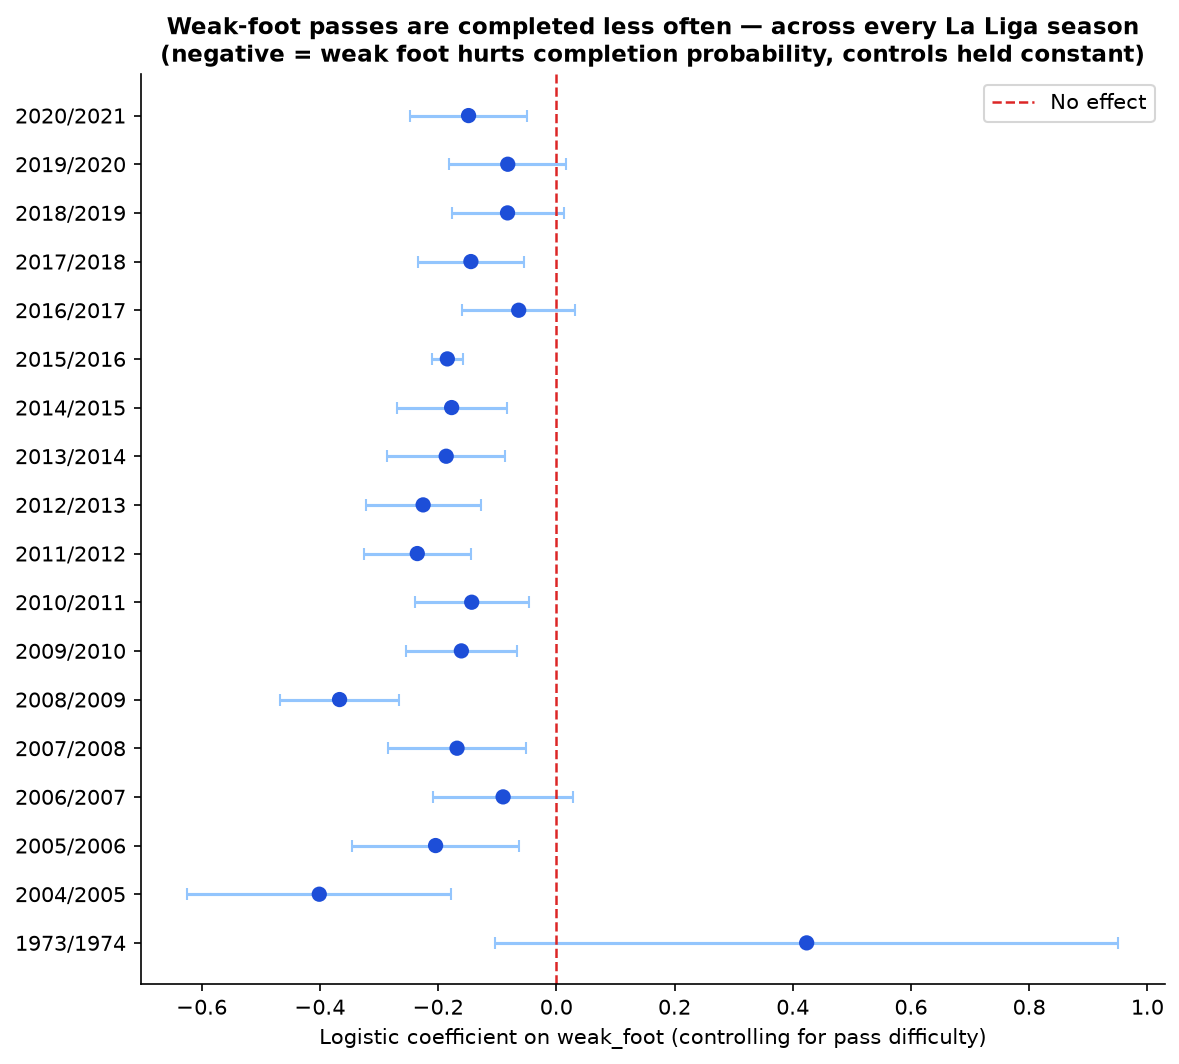
\includegraphics[width=0.85\textwidth]{weak_foot_forest_plot.png}
\caption{Controlled weak-foot logistic coefficient per season (95\% CI).
Negative values mean weak-foot passes are less likely to complete after
controlling for pass difficulty.}
\label{fig:forest}
\end{figure}

\subsection{Finding 2: calibration collapses on rare pass types}
Per-season AUC lies between 0.85 and 0.91
(\url{calibration_summary_by_season.csv}), confirming the model is
strong globally. Pooling held-out predictions across seasons and
stratifying by type tells a different story (Table~\ref{tab:cal},
Figure~\ref{fig:cal}). Ordinary passes (n~=~173\,215) are near-perfectly
calibrated (ECE~=~0.003, Brier~=~0.092). Calibration then degrades
monotonically with scarcity: Cross (n~=~4\,057, ECE~=~0.017), Switch
(n~=~4\,689, ECE~=~0.022), Through ball (n~=~1\,204, ECE~=~0.043,
Brier~=~0.226). (Cut-back: n~=~145, ECE~=~0.070, shown for completeness.)
The model is systematically overconfident on every rare
type, and the degradation scales with sample size rather than with any
intrinsic property of the type.
\begin{table}[h]
\centering
\begin{tabular}{lrrrrr}
\toprule
Type & n & Actual rate & Predicted rate & Brier & ECE \\
\midrule
Ordinary & 173215 & 0.812 & 0.814 & 0.092 & 0.003 \\
Cross & 4057 & 0.289 & 0.284 & 0.185 & 0.017 \\
Switch & 4689 & 0.737 & 0.739 & 0.132 & 0.022 \\
Through ball & 1204 & 0.402 & 0.403 & 0.226 & 0.043 \\
Cut-back & 145 & 0.545 & 0.567 & 0.179 & 0.070 \\
\bottomrule
\end{tabular}
\caption{Calibration by pass type, pooled across seasons
(\url{calibration_summary_by_pass_type.csv}). Through balls are
$15\times$ worse calibrated than Ordinary passes.}
\label{tab:cal}
\end{table}
\begin{figure}[h]
\centering
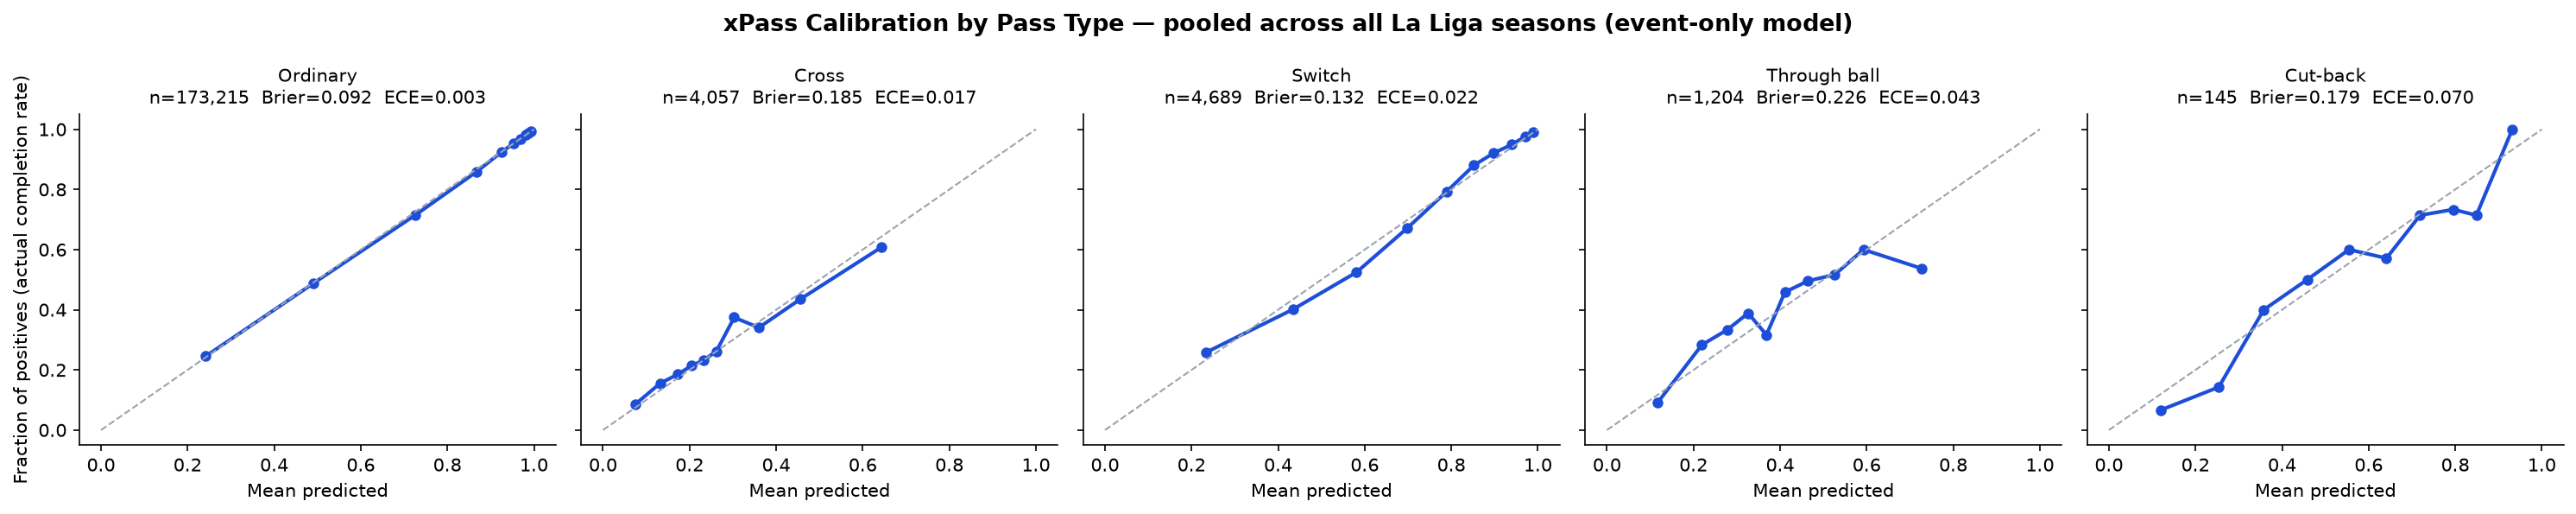
\includegraphics[width=\textwidth]{calibration_by_pass_type.png}
\caption{Reliability diagrams per pass type, pooled across all seasons
(event-only model). Ordinary passes hug the diagonal; rare types deviate.}
\label{fig:cal}
\end{figure}

\subsection{Finding 2b: equal-n downsampling splits scarcity from type effects}
Naive ECE comparisons conflate two things: true miscalibration and the
estimator's own noise, since 10-bin ECE measured on hundreds of points is
upward-biased even for a calibrated model. Table~\ref{tab:down} removes
the confound by scoring Ordinary passes at exactly each rare type's n
(200 resamples; five largest seasons, $\sim$100k Ordinary pooled).
Two facts emerge. First, scarcity dominates: Ordinary ECE inflates roughly
eightfold going from full pool (0.004) to n~=~591 (0.031, 95\% interval
0.019--0.048), since most of the rare-type gap is sample size plus binning
noise. Second, a residual type effect survives equal n: Through balls
(0.046) calibrate about 1.5$\times$ worse than Ordinary at n~=~591
(0.031), Switch (0.032) over 2$\times$ worse at n~=~2754 (0.014), and
Cross (0.019) mildly worse at n~=~2563 (0.015). Scarcity explains the bulk of the
miscalibration, but rare types carry an additional intrinsic penalty,
consistent with their lower base rates and contested nature, that more
data alone would shrink but not erase.
\begin{table}[h]
\centering
\begin{tabular}{lrrrr}
\toprule
Subset & n & Brier & ECE & 95\% interval \\
\midrule
Ordinary (full) & 100681 & 0.097 & 0.004 & n/a \\
Ordinary@n=10000 & 10000 & n/a & 0.008 & 0.004--0.013 \\
Ordinary@n=2754 & 2754 & n/a & 0.014 & 0.008--0.022 \\
Switch & 2754 & 0.129 & 0.032 & n/a \\
Ordinary@n=2563 & 2563 & n/a & 0.015 & 0.009--0.024 \\
Cross & 2563 & 0.183 & 0.019 & n/a \\
Ordinary@n=591 & 591 & n/a & 0.031 & 0.019--0.048 \\
Through ball & 591 & 0.228 & 0.046 & n/a \\
\bottomrule
\end{tabular}
\caption{Equal-n downsampling: Ordinary ECE at each rare type's sample size
(mean over 200 resamples) versus the rare type's actual ECE
(\url{downsample_summary.csv}). Scarcity explains most of the gap; a residual gap of up to $\sim$2$\times$ remains.}
\label{tab:down}
\end{table}

\subsection{Finding 3: ablation: footedness effects are small and inconsistent}
\label{sec:ablation}
Figure~\ref{fig:abl} compares the three footedness variants. No variant wins everywhere: the current
feature set is best on Cross (ECE 0.017 versus 0.021/0.019) but not on Switch, where no-footedness is best (0.021 versus 0.022/0.024), nor on Through balls, where full-interactions leads (0.039 versus 0.043/0.044); while Ordinary passes are identical (ECE~=~0.003) everywhere and the mean hard-type ECE differs only in the third decimal (0.027--0.028). In other words, footedness carries signal, but with only a few thousand rare-type examples the model cannot reliably attribute it per type: adding interactions just moves the error around. Missing footedness features are not the cause of the
calibration gap.
\begin{figure}[h]
\centering
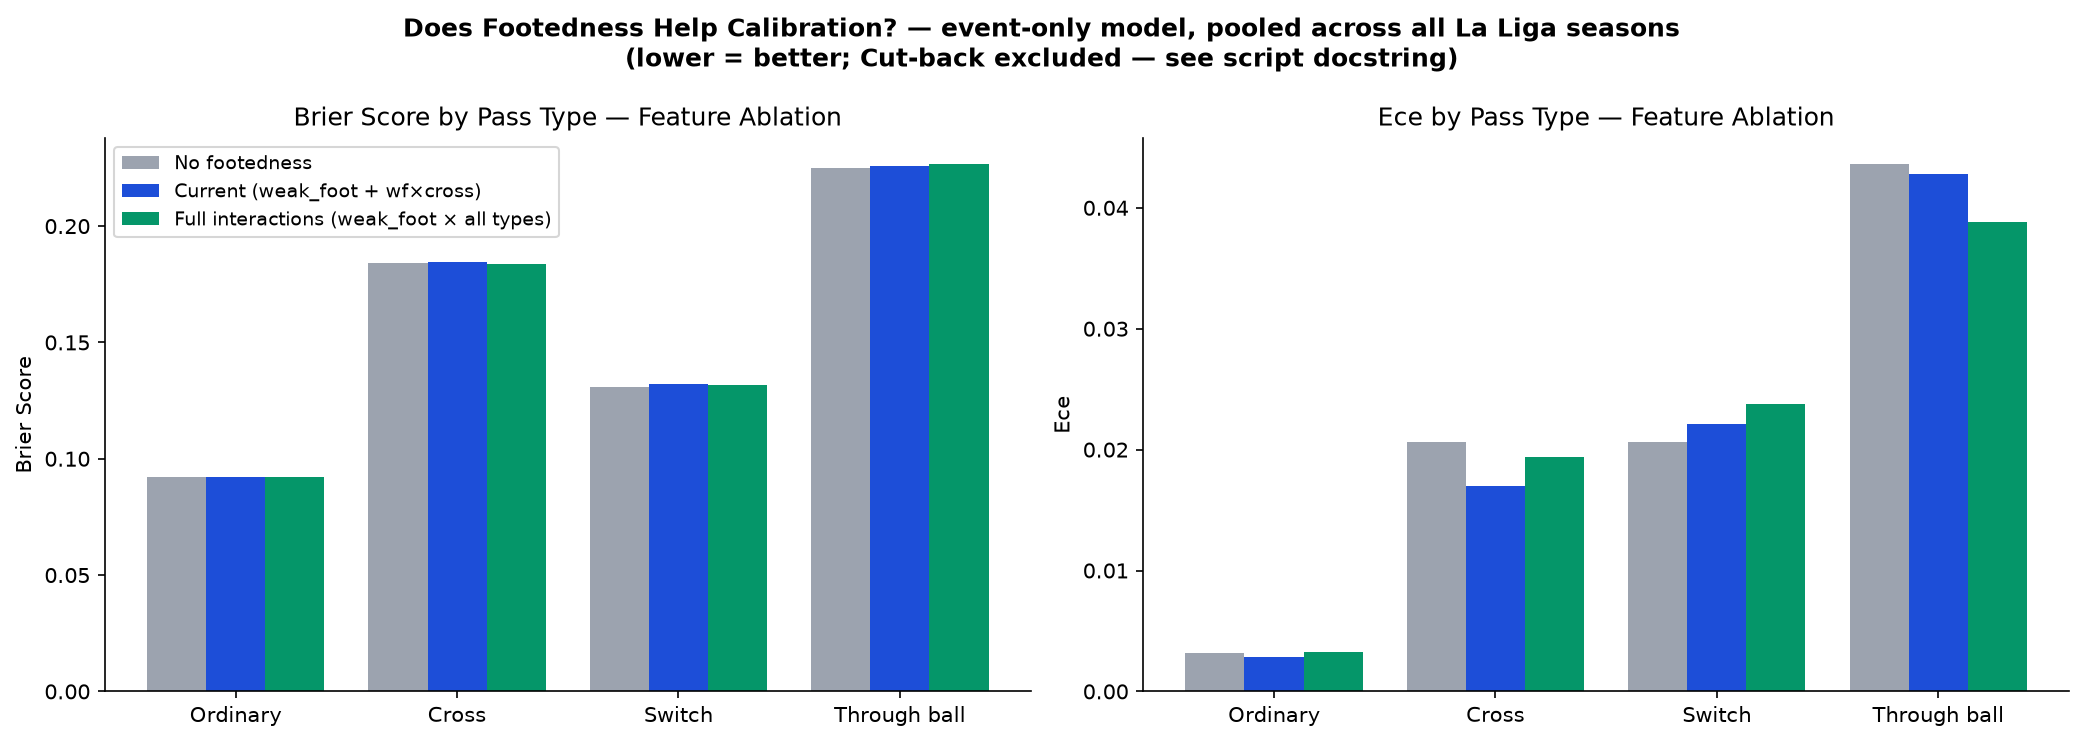
\includegraphics[width=\textwidth]{ablation_calibration_by_pass_type.png}
\caption{Ablation: Brier score and ECE per pass type for the three
footedness variants (lower is better; pooled across seasons).}
\label{fig:abl}
\end{figure}

\subsection{Finding 3b: reweighting rare types hurts calibration}
Since scarcity is the suspect, the natural fix is to upweight rare pass
types during training. Table~\ref{tab:weight} shows this backfires.
Inverse-frequency weighting degrades ECE on Ordinary (0.004 to 0.009),
Cross (0.019 to 0.037), and especially Through balls (0.046 to 0.103),
while overall AUC falls from 0.896 to 0.889; only Switch improves
slightly (ECE 0.032 to 0.024, Brier 0.129 to 0.121), and the milder
square-root weighting shows the same pattern in muted form. The reason is
structural: calibration means predicted probabilities match observed base
rates, and reweighting deliberately distorts the training distribution,
so the model learns shifted base rates. Weighting can aid discrimination
under imbalance, but it works against calibration by construction, so a
weighted model would need its own recalibration step afterward. This is
the third attempted fix (after foot features and their interactions) to
fail on rare types in exactly the way scarcity predicts. Full numbers are
in \url{weighted_summary.csv}.
\begin{table}[h]
\centering
\begin{tabular}{lrrrrrr}
\toprule
Type & n & \multicolumn{2}{c}{Unweighted} & \multicolumn{2}{c}{Inv.\ weighted} \\
 & & Brier & ECE & Brier & ECE \\
\midrule
Ordinary & 100681 & 0.097 & 0.004 & 0.101 & 0.009 \\
Switch & 2754 & 0.129 & 0.032 & 0.121 & 0.024 \\
Cross & 2563 & 0.183 & 0.019 & 0.187 & 0.037 \\
Through ball & 591 & 0.228 & 0.046 & 0.239 & 0.103 \\
\bottomrule
\end{tabular}
\caption{Type-weighted training versus unweighted, pooled held-out
predictions over the five largest cached seasons
(\url{weighted_summary.csv}). Weighting helps only Switch, marginally,
and harms everything else.}
\label{tab:weight}
\end{table}

\subsection{Finding 4: recalibration fails on every rare type, confirming scarcity}
Isotonic recalibration is a flexible monotone correction: it thrives on
large samples and overfits small ones, which makes it a diagnostic tool
here. Figure~\ref{fig:recal} shows before/after reliability per type, and the correction fails everywhere it is needed. On Through balls (evaluation n~=~602) ECE rises from 0.054 to 0.074; on Cross (n~=~2\,029) from 0.012 to 0.021; on Switch (n~=~2\,345) from 0.021 to 0.028; Ordinary (n~=~86\,680) is unchanged (ECE~=~0.003 to 0.002). Brier scores move the same way. That no rare type has enough held-out data to fit even a one-dimensional correction is itself the result: the failure is uniform, exactly as sample scarcity predicts, and it rules out recalibration as a cheap fix.
\begin{figure}[h]
\centering
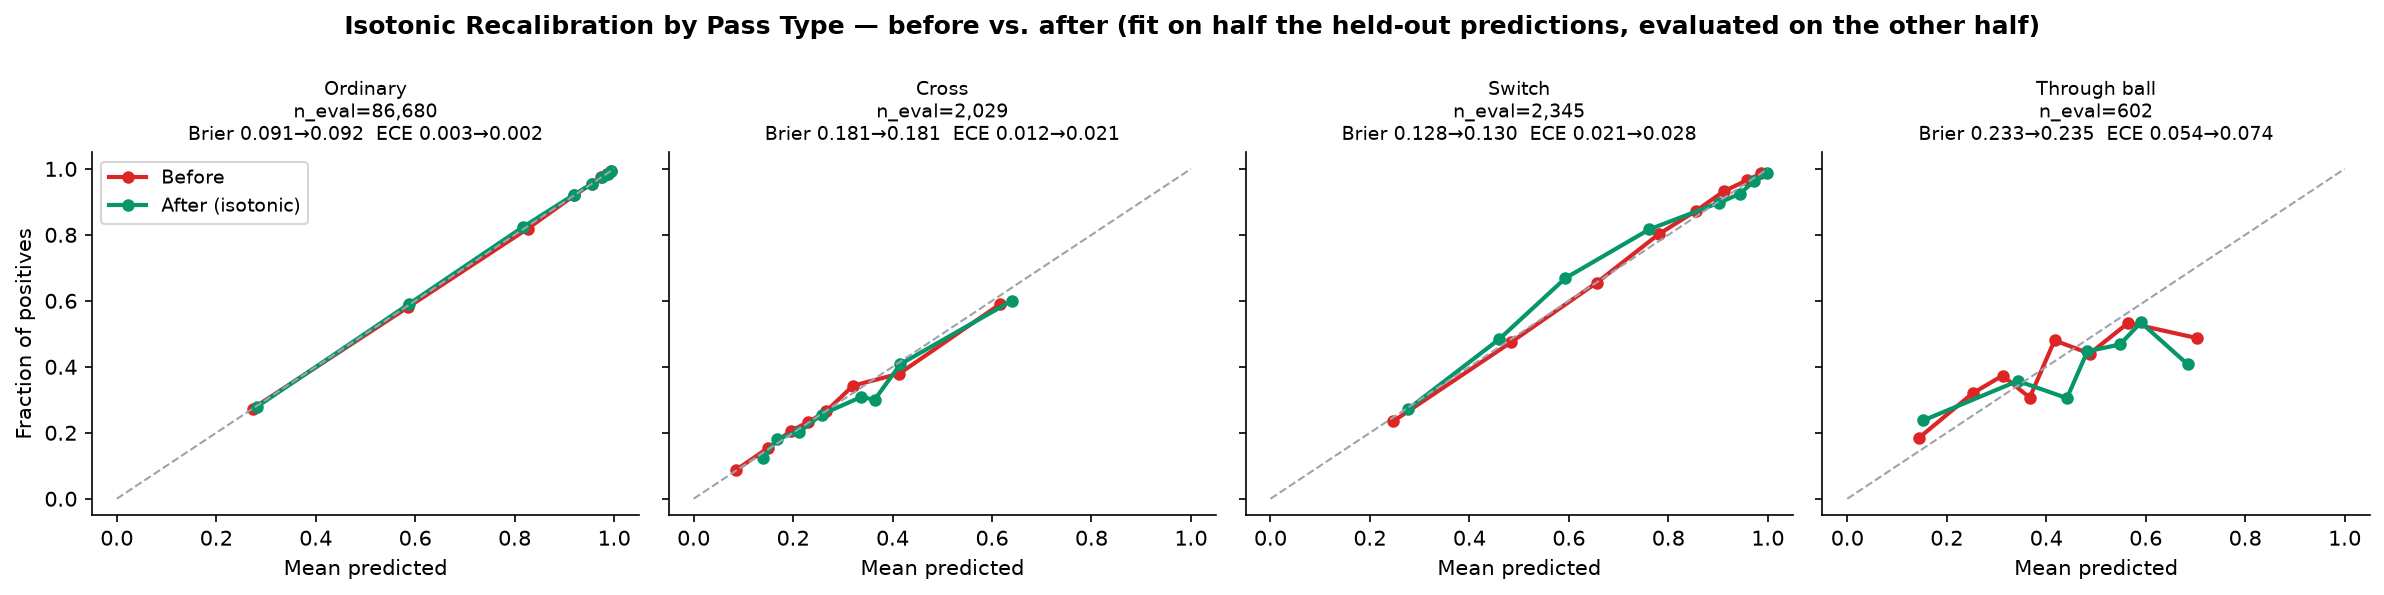
\includegraphics[width=\textwidth]{recalibration_before_after.png}
\caption{Isotonic recalibration before versus after, per pass type (fit on
half the pooled held-out predictions, evaluated on the other half).}
\label{fig:recal}
\end{figure}

\subsection{Bonus: 2020/21 event-only versus 360-enriched}
The \url{all_seasons.py} 360 flag re-runs the notebook's
360-enriched comparison for the one season with freeze-frame data (code path available; figure omitted from \url{poster_outputs}). Adding
defender distances, lane occupancy, and visible-player counts does not
change the weak-foot story or the rare-type pattern, consistent with the
conclusion that context features are not the binding constraint.

\section{Discussion}
Four regularities point the same way. First, the weak-foot penalty is
real and stable across tactical eras, yet the model already observes it
and still miscalibrates rare types. Second, calibration error orders
itself by sample size across types, and equal-n downsampling shows
Ordinary passes degrade roughly eightfold when starved to rare-type sizes,
though a residual gap of up to $\sim$2$\times$ survives matching, so rare
types are intrinsically harder too. Third, neither richer footedness
features nor type-reweighting fix the gap: reweighting even harms
calibration, as theory predicts for base-rate-distorting weights.
Fourth, a flexible recalibration fails on
every rare type while leaving Ordinary untouched. Together they imply
that collecting more examples of rare passes, or borrowing strength
across them hierarchically, will help more than further feature
engineering on the same examples. Practically, xPass can already be
personalised with footedness for scouting and player evaluation
(a $\sim$15--20\% odds adjustment is material for high-volume crossers of
the wrong foot), but its probabilities on crosses, switches, and
through balls should be presented with uncertainty until recalibrated on
adequate samples.

\section{Limitations and future work}
Usage-inferred footedness mislabels some players and the FIFA validation
covers 2020/21 only. Body orientation, receiver availability, scoreline
and match time, and possession-sequence context are unmodelled. In
particular, following Anzer and Bauer (2022), our event-only features never
identify the intended receiver: the true target of a pass can only be
recovered by modelling the ball trajectory from physics together with rich
spatio-temporal tracking of all players, data our pipeline does not use.
Early
seasons overweight a single club. Future work should add game-state and
sequential features (e.g.\ LSTM or graph-based encodings of the
possession), richer player technical attributes, and hierarchical or
empirical-Bayes calibration that pools rare types instead of fitting each
in isolation.

\section{Reproducibility}
python \url{all_seasons.py} (full multi-season run; --seasons
flags allow quick tests; --with-360 adds the bonus) followed by
python \url{calibration_study.py} regenerates every figure and CSV in
\url{poster_outputs/}, and python \url{weighted_study.py}
regenerates the weighting comparison (\url{weighted_summary.csv});
see the README for dependencies. The frozen
analysis notebook, foot-source scrapers, the \url{xPass.ipynb} scratch
check behind the 1973/74 exclusion, and the early single-season figures
and dashboard are preserved in \url{archive/}.

\begin{thebibliography}{9}
\bibitem{anzer2022} Anzer, G.\ and Bauer, P.\ (2022). Expected passes:
Determining the difficulty of a pass in football (soccer) using
spatio-temporal data. \textit{Data Mining and Knowledge Discovery}.
\bibitem{arbues2020} Arbu\'es-Sang\"uesa, A.\ et al.\ (2020). Using
player's body-orientation to model pass feasibility in soccer.
\textit{Proc.\ IEEE/CVF CVPR Workshops}.
\bibitem{szczepanski2016} Szczepa\'nski, \L.\ and McHale, I.\ (2016).
Beyond completion rate: Evaluating the passing ability of footballers.
\textit{J.\ Royal Statistical Society Series A}.
\bibitem{robberechts2023} Robberechts, P.\ et al.\ (2023). Creativity /
Un-xPass extensions to pass evaluation.
\bibitem{rahimian2024} Rahimian, P.\ et al.\ (2024). Pass receiver and
outcome prediction using temporal graph networks. In \textit{ML and Data
Mining for Sports Analytics}.
\bibitem{takamido2025} Takamido, R.\ et al.\ (2025). PassAI: An
explainable machine learning framework for predicting soccer pass
outcomes using multimodal match data. \textit{IEEE Access}.
\end{thebibliography}

\end{document}
